%\documentclass[hyperref={pdfpagelabels=false},slidetop,9pt]{beamer}
\documentclass[slidetop,8pt]{beamer}
\usepackage[T1]{fontenc}
\usepackage[utf8]{inputenc}
\newcommand{\id}{54}
\newcommand{\nom}{Liaisons mécaniques}
\newcommand{\sequence}{04}
\newcommand{\num}{01}
\newcommand{\type}{TP}
\newcommand{\descrip}{Modélisation d'un solide. Comportement des liaisons mécaniques. Modéliser les mécanismes du laboratoire par un schéma cinématique, paramétré.}
\newcommand{\competences}{A3-C4: Analyse d'architecture et de comportement \\ &  Mod1-C1: Isolement d'un solide ou d'un système de solides \\ &  Mod2-C10-1: Modèle de solide indéformable \\ &  Mod2-C11: Modélisation géométrique et cinématique des mouvements entre solides indéformables \\ &  Mod2-C12: Modélisation cinématique des liaisons entre solides \\ &  Mod2-C15: Modélisation des actions mécaniques \\ &  Rés-C6: Utilisation d'un solveur ou d'un logiciel multi physique \\ &  Com1-C1: Différents descripteurs introduits dans le programme \\ &  Com2-C4: Outils de communication}
\newcommand{\nbcomp}{9}
\newcommand{\systemes}{Plateforme Stewart}
\newcommand{\systemessansaccent}{Plateforme Stewart}
\newcommand{\ilot}{2}
\newcommand{\ilotstr}{02}
\newcommand{\dossierilot}{\detokenize{Ilot_02 Plateforme Stewart}}
\newcommand{\imageun}{Plateforme}

\newcommand{\urlsysteme}{\href{https://www.costadoat.fr/systeme/57}{Ressources système}}
\newcommand{\matlabsimscape}{\href{https://github.com/Costadoat/Sciences-Ingenieur/raw/master/Systemes/Plateforme Stewart/Plateforme_Stewart_Simscape.zip}{Modèle Simscape}}
\newcommand{\solidworks}{\href{https://github.com/Costadoat/Sciences-Ingenieur/raw/master/Systemes/Plateforme Stewart/Plateforme_Stewart_Solidworks.zip}{Modèle Solidworks}}
\newcommand{\edrawings}{\href{https://github.com/Costadoat/Sciences-Ingenieur/raw/master/Systemes/Plateforme Stewart/Plateforme_Stewart.EASM}{Modèle eDrawings}}
\newcommand{\test}{Stewart_param1}
\newcommand{\testi}{Stewart_param2}
\newcommand{\testii}{Stewart_param3}
\newcommand{\testiii}{Stewart_param4}
\newcommand{\testiiii}{Stewart_euler}
\usepackage{etex}
\usepackage{tikz}
\usepackage[european]{circuitikz}
\usepackage{pgf}
\usepackage[all]{xy}
\usepackage{pgfpages}
\usepackage{graphbox}
\usepackage{pdfpages}
\usepackage[adobe-utopia]{mathdesign}
\usepackage{ifthen}
\usepackage{cancel}
\usepackage{framed}
\usepackage{subfig}
\usepackage{tabularx}
\usepackage{setspace}
\usepackage{soul}
\usepackage{schemabloc}
\usepackage{eqnarray}
\usepackage[dot, phantomtext]{dashundergaps}
\usepackage{media9}
\usepackage{multimedia}
\usepackage{textcomp}

\author{Renaud Costadoat}
\institute{Lycée Dorian}

\usepackage{multido}
\usepackage{multirow}
\usepackage{multicol} % Portions de texte en colonnes
\usepackage{flafter}%floatants après la référence

\usepackage{color}
\usepackage{xcolor}
\usepackage{colortbl}

\usepackage[gen]{eurosym}
\usepackage{tikz}
%\usepackage{pstricks,pst-node,pst-tree,pst-solides3d}
\usepackage{lmodern}
\usepackage[francais]{babel}
\usepackage{pslatex}
\usetheme{renaud}
\usepackage{times}
\usepackage{amsmath}
\usepackage{verbatim}
\usepackage{moreverb}
%\usetikzlibrary{arrows,shapes}
\usepackage{graphicx}
\usepackage{psfrag}
\usepackage{wrapfig}
\usepackage{etoolbox}

\definecolor{gris25}{gray}{0.75}
\definecolor{bleu}{RGB}{18,33,98}
\definecolor{bleuf}{RGB}{42,94,171}
\definecolor{bleuc}{RGB}{231,239,247}
\definecolor{rougef}{RGB}{185,18,27}
\definecolor{rougec}{RGB}{255,188,204}%255,230,231
\definecolor{vertf}{RGB}{103,126,82}
\definecolor{vertc}{RGB}{220,255,191}

\setlength\parindent{24pt}
\parskip 7.2pt
\parindent 8pt

\newenvironment{rem}[1][\hsize]%
{%
    \def\FrameCommand
   {%
\rotatebox{90}{\textit{\textsf{Remarque}}} 
       {\color{bleuf}\vrule width 3pt}%
       \hspace{0pt}%must no space.
       \fboxsep=\FrameSep\colorbox{bleuc}%
  }%
    \MakeFramed{\hsize#1\advance\hsize-\width\FrameRestore}%
}%
{\endMakeFramed}%


\newenvironment{savoir}[1][\hsize]%
{%
    \def\FrameCommand
    {%
\rotatebox{90}{\textit{\textsf{Savoir}}} 
        {\color{bleuf}\vrule width 3pt}%
        \hspace{0pt}%must no space.
        \fboxsep=\FrameSep\colorbox{bleuc}%
    }%
    \MakeFramed{\hsize#1\advance\hsize-\width\FrameRestore}%
}%
{\endMakeFramed}%

\newenvironment{prob}[1][\hsize]%
{%
    \def\FrameCommand%
    {%
\rotatebox{90}{\textit{\textsf{Problematique}}} 
        {\color{rougef}\vrule width 3pt}%
        \hspace{0pt}%must no space.
        \fboxsep=\FrameSep\colorbox{rougec}%
    }%
    \MakeFramed{\hsize#1\advance\hsize-\width\FrameRestore}%
}%
{\endMakeFramed}%

\newenvironment{obj}[1][\hsize]%
{%
    \def\FrameCommand%
    {%
\rotatebox{90}{\textit{\textsf{Objectif}}} 
        {\color{vertf}\vrule width 3pt}%
        \hspace{0pt}%must no space.
        \fboxsep=\FrameSep\colorbox{vertc}%
    }%
    \MakeFramed{\hsize#1\advance\hsize-\width\FrameRestore}%
}%
{\endMakeFramed}%

\newenvironment{defi}[1][\hsize]%
{%
    \def\FrameCommand%
    {%
\rotatebox{90}{\textit{\textsf{Definition}}} 
        {\color{bleuf}\vrule width 3pt}%
        \hspace{0pt}%must no space.
        \fboxsep=\FrameSep\colorbox{rougec}%
    }%
    \MakeFramed{\hsize#1\advance\hsize-\width\FrameRestore}%
}%
{\endMakeFramed}%


\newenvironment{hypo}[1][\hsize]%
{%
    \def\FrameCommand%
    {%
\rotatebox{90}{\textit{\textsf{Hypothèse\\}}} 
        {\color{bleuf}\vrule width 3pt}%
        \hspace{0pt}%must no space.
        \fboxsep=\FrameSep\colorbox{bleuc}%
    }%
    \MakeFramed{\hsize#1\advance\hsize-\width\FrameRestore}%
}%
{\endMakeFramed}%


\newenvironment{prop}[1][\hsize]%
{%
    \def\FrameCommand%
    {%
\rotatebox{90}{\textit{\textsf{Propriété}}} 
        {\color{bleuf}\vrule width 3pt}%
        \hspace{0pt}%must no space.
        \fboxsep=\FrameSep\colorbox{bleuc}%
    }%
    \MakeFramed{\hsize#1\advance\hsize-\width\FrameRestore}%
}%
{\endMakeFramed}%

\newenvironment{props}[1][\hsize]%
{%
    \def\FrameCommand%
    {%
\rotatebox{90}{\textit{\textsf{Propriétés}}} 
        {\color{bleuf}\vrule width 3pt}%
        \hspace{0pt}%must no space.
        \fboxsep=\FrameSep\colorbox{bleuc}%
    }%
    \MakeFramed{\hsize#1\advance\hsize-\width\FrameRestore}%
}%
{\endMakeFramed}%

\newenvironment{exemple}[1][\hsize]%
{%
    \def\FrameCommand%
    {%
\rotatebox{90}{\textit{\textsf{Exemple}}} 
        {\color{vertf}\vrule width 3pt}%
        \hspace{0pt}%must no space.
        \fboxsep=\FrameSep\colorbox{vertc}%
    }%
    \MakeFramed{\hsize#1\advance\hsize-\width\FrameRestore}%
}%
{\endMakeFramed}%

\newenvironment{resultat}[1][\hsize]%
{%
    \def\FrameCommand%
    {%
\rotatebox{90}{\textit{\textsf{Résultat}}} 
        {\color{rougef}\vrule width 3pt}%
%        {\color{bleuf}\vrule width 3pt}%
        \hspace{0pt}%must no space.
        \fboxsep=\FrameSep\colorbox{rougec}%
    }%
    \MakeFramed{\hsize#1\advance\hsize-\width\FrameRestore}%
}%
{\endMakeFramed}%

\newenvironment{methode}[1][\hsize]%
{%
    \def\FrameCommand%
    {%
\rotatebox{90}{\textit{\textsf{Méthode\\}}} 
        {\color{rougef}\vrule width 3pt}%
        \hspace{0pt}%must no space.
        \fboxsep=\FrameSep\colorbox{rougec}%
    }%
    \MakeFramed{\hsize#1\advance\hsize-\width\FrameRestore}%
}%
{\endMakeFramed}%

\newenvironment{theo}[1][\hsize]%
{%
    \def\FrameCommand%
    {%
\rotatebox{90}{\textit{\textsf{Théorème\\}}} 
        {\color{rougef}\vrule width 3pt}%
        \hspace{0pt}%must no space.
        \fboxsep=\FrameSep\colorbox{rougec}%
    }%
    \MakeFramed{\hsize#1\advance\hsize-\width\FrameRestore}%
}%
{\endMakeFramed}%

\newenvironment{warn}[1][\hsize]%
{%
    \def\FrameCommand%
    {%
\rotatebox{90}{\textit{\textsf{Attention\\}}} 
        {\color{rougef}\vrule width 3pt}%
        \hspace{0pt}%must no space.
        \fboxsep=\FrameSep\colorbox{rougec}%
    }%
    \MakeFramed{\hsize#1\advance\hsize-\width\FrameRestore}%
}%
{\endMakeFramed}%

% \usepackage{pstricks}
%\usepackage{minitoc}
% \setcounter{minitocdepth}{4}

\setcounter{tocdepth}{2}

% \mtcselectlanguage{french} 

%\usepackage{draftcopy}% "Brouillon"
% \usepackage{floatflt}
\usepackage{psfrag}
%\usepackage{listings} % Permet d'insérer du code de programmation
\renewcommand{\baselinestretch}{1.2}

% Changer la num�rotation des figures :
% ------------------------------------
% \makeatletter
% \renewcommand{\thefigure}{\ifnum \c@section>\z@ \thesection.\fi
%  \@arabic\c@figure}
% \@addtoreset{figure}{section}
% \makeatother
 


%%%%%%%%%%%%
% Définition des vecteurs %
%%%%%%%%%%%%
 \newcommand{\vect}[1]{\overrightarrow{#1}}

%%%%%%%%%%%%
% Définition des torseusr %
%%%%%%%%%%%%

 \newcommand{\torseur}[1]{%
\left\{{#1}\right\}
}

\newcommand{\torseurcin}[3]{%
\left\{\mathcal{#1} \left(#2/#3 \right) \right\}
}

\newcommand{\torseurstat}[3]{%
\left\{\mathcal{#1} \left(#2\rightarrow #3 \right) \right\}
}

 \newcommand{\torseurc}[8]{%
%\left\{#1 \right\}=
\left\{
{#1}
\right\}
 = 
\left\{%
\begin{array}{cc}%
{#2} & {#5}\\%
{#3} & {#6}\\%
{#4} & {#7}\\%
\end{array}%
\right\}_{#8}%
}

 \newcommand{\torseurcol}[7]{
\left\{%
\begin{array}{cc}%
{#1} & {#4}\\%
{#2} & {#5}\\%
{#3} & {#6}\\%
\end{array}%
\right\}_{#7}%
}

 \newcommand{\torseurl}[3]{%
%\left\{\mathcal{#1}\right\}_{#2}=%
\left\{%
\begin{array}{l}%
{#1} \\%
{#2} %
\end{array}%
\right\}_{#3}%
}

 \newcommand{\vectv}[3]{%
\vect{V\left( {#1} \in {#2}/{#3}\right)}
}


\newcommand{\vectf}[2]{%
\vect{R\left( {#1} \rightarrow {#2}\right)}
}

\newcommand{\vectm}[3]{%
\vect{\mathcal{M}\left( {#1}, {#2} \rightarrow {#3}\right)}
}


 \newcommand{\vectg}[3]{%
\vect{\Gamma \left( {#1} \in {#2}/{#3}\right)}
}

 \newcommand{\vecto}[2]{%
\vect{\Omega\left( {#1}/{#2}\right)}
}

\newcommand{\reponse}[1][4]
{
\multido{}{#1}
{
\begin{center}
\makebox[0.9\linewidth]{\dotfill} \end{center}
}}


% }$$\left\{\mathcal{#1} \right\}_{#2} =%
% \left\{%
% \begin{array}{c}%
%  #3 \\%
%  #4 %
% \end{array}%
% \right\}_{#5}}


%  ------------------------------------------
% | Modification du formatage des sections : | 
%  ------------------------------------------

% Grands titres :
% ---------------

\newcommand{\titre}[1]{%
\begin{center}
      \bigskip
      \rule{\textwidth}{1pt}
      \par\vspace{0.1cm}
      
      \textbf{\large #1}
      \par\rule{\textwidth}{1pt}
    \end{center}
    \bigskip
  }

% Supprime le numéro du chapitre dans la numérotation des sections:
% -----------------------------------------------------------------
\makeatletter
\renewcommand{\thesection}{\@arabic\c@section}
\makeatother


% \titleformat{\chapter}[display]
% {\normalfont\Large\filcenter}
% {}
% {1pc}
% {\titlerule[1pt]
%   \vspace{1pc}%
%   \Huge}[\vspace{1ex}%
% \titlerule]


%%%% Chapitres Comme PY Pechard %%%%%%%%%
% numéro du chapitre
\DeclareFixedFont{\chapnumfont}{OT1}{phv}{b}{n}{80pt}
% pour le mot " Chapitre "
\DeclareFixedFont{\chapchapfont}{OT1}{phv}{m}{it}{40pt}
% pour le titre
\DeclareFixedFont{\chaptitfont}{T1}{phv}{b}{n}{25pt}

\definecolor{gris}{gray}{0.75}
\setbeamertemplate{section in toc}[sections numbered]

\newlength{\RoundedBoxWidth}
\newsavebox{\GrayRoundedBox}
\newenvironment{GrayBox}[1][\dimexpr\textwidth-4.5ex]%
   {\setlength{\RoundedBoxWidth}{\dimexpr#1}
    \begin{lrbox}{\GrayRoundedBox}
       \begin{minipage}{\RoundedBoxWidth}}%
   {   \end{minipage}
    \end{lrbox}
    \begin{center}
    \begin{tikzpicture}%
       \draw node[draw=bleuf,fill=bleuc,rounded corners,%
             inner sep=2ex,text width=\RoundedBoxWidth]%
             {\usebox{\GrayRoundedBox}};
    \end{tikzpicture}
    \end{center}}
    
\ifdef{\prive}{\pgfpagesuselayout{2 on 1}[a4paper,border shrink=0mm]}
\ifdef{\prive}{\setbeamertemplate{navigation symbols}{}}
\setbeamertemplate{itemize item}[ball]
%\setbeamertemplate{blocks}[rounded]%[shadow=true]
\setbeamercolor{block title}{fg=white,bg=grisf}        % titre block normal 
\setbeamercolor{block body}{fg=grisf,bg=grisc!50}      % corps block normal
\setbeamercolor{block body alerted}{fg=white,bg=warning}   % idem pour un block alerte

\title{\nom}
\date{S\sequence \ - \type\num}

\begin{document}
\shorthandoff{:!}
\bibliographystyle{abbrvnat-fr}

\usebackgroundtemplate%
{%
    \centering
\includegraphics[width=\paperwidth]{../../img/fond2}%
}

{
\setbeamertemplate{navigation symbols}{}
\setbeamertemplate{headline}[pagetitre]
\setbeamertemplate{footline}[pagetitre]
\usebackgroundtemplate{\centering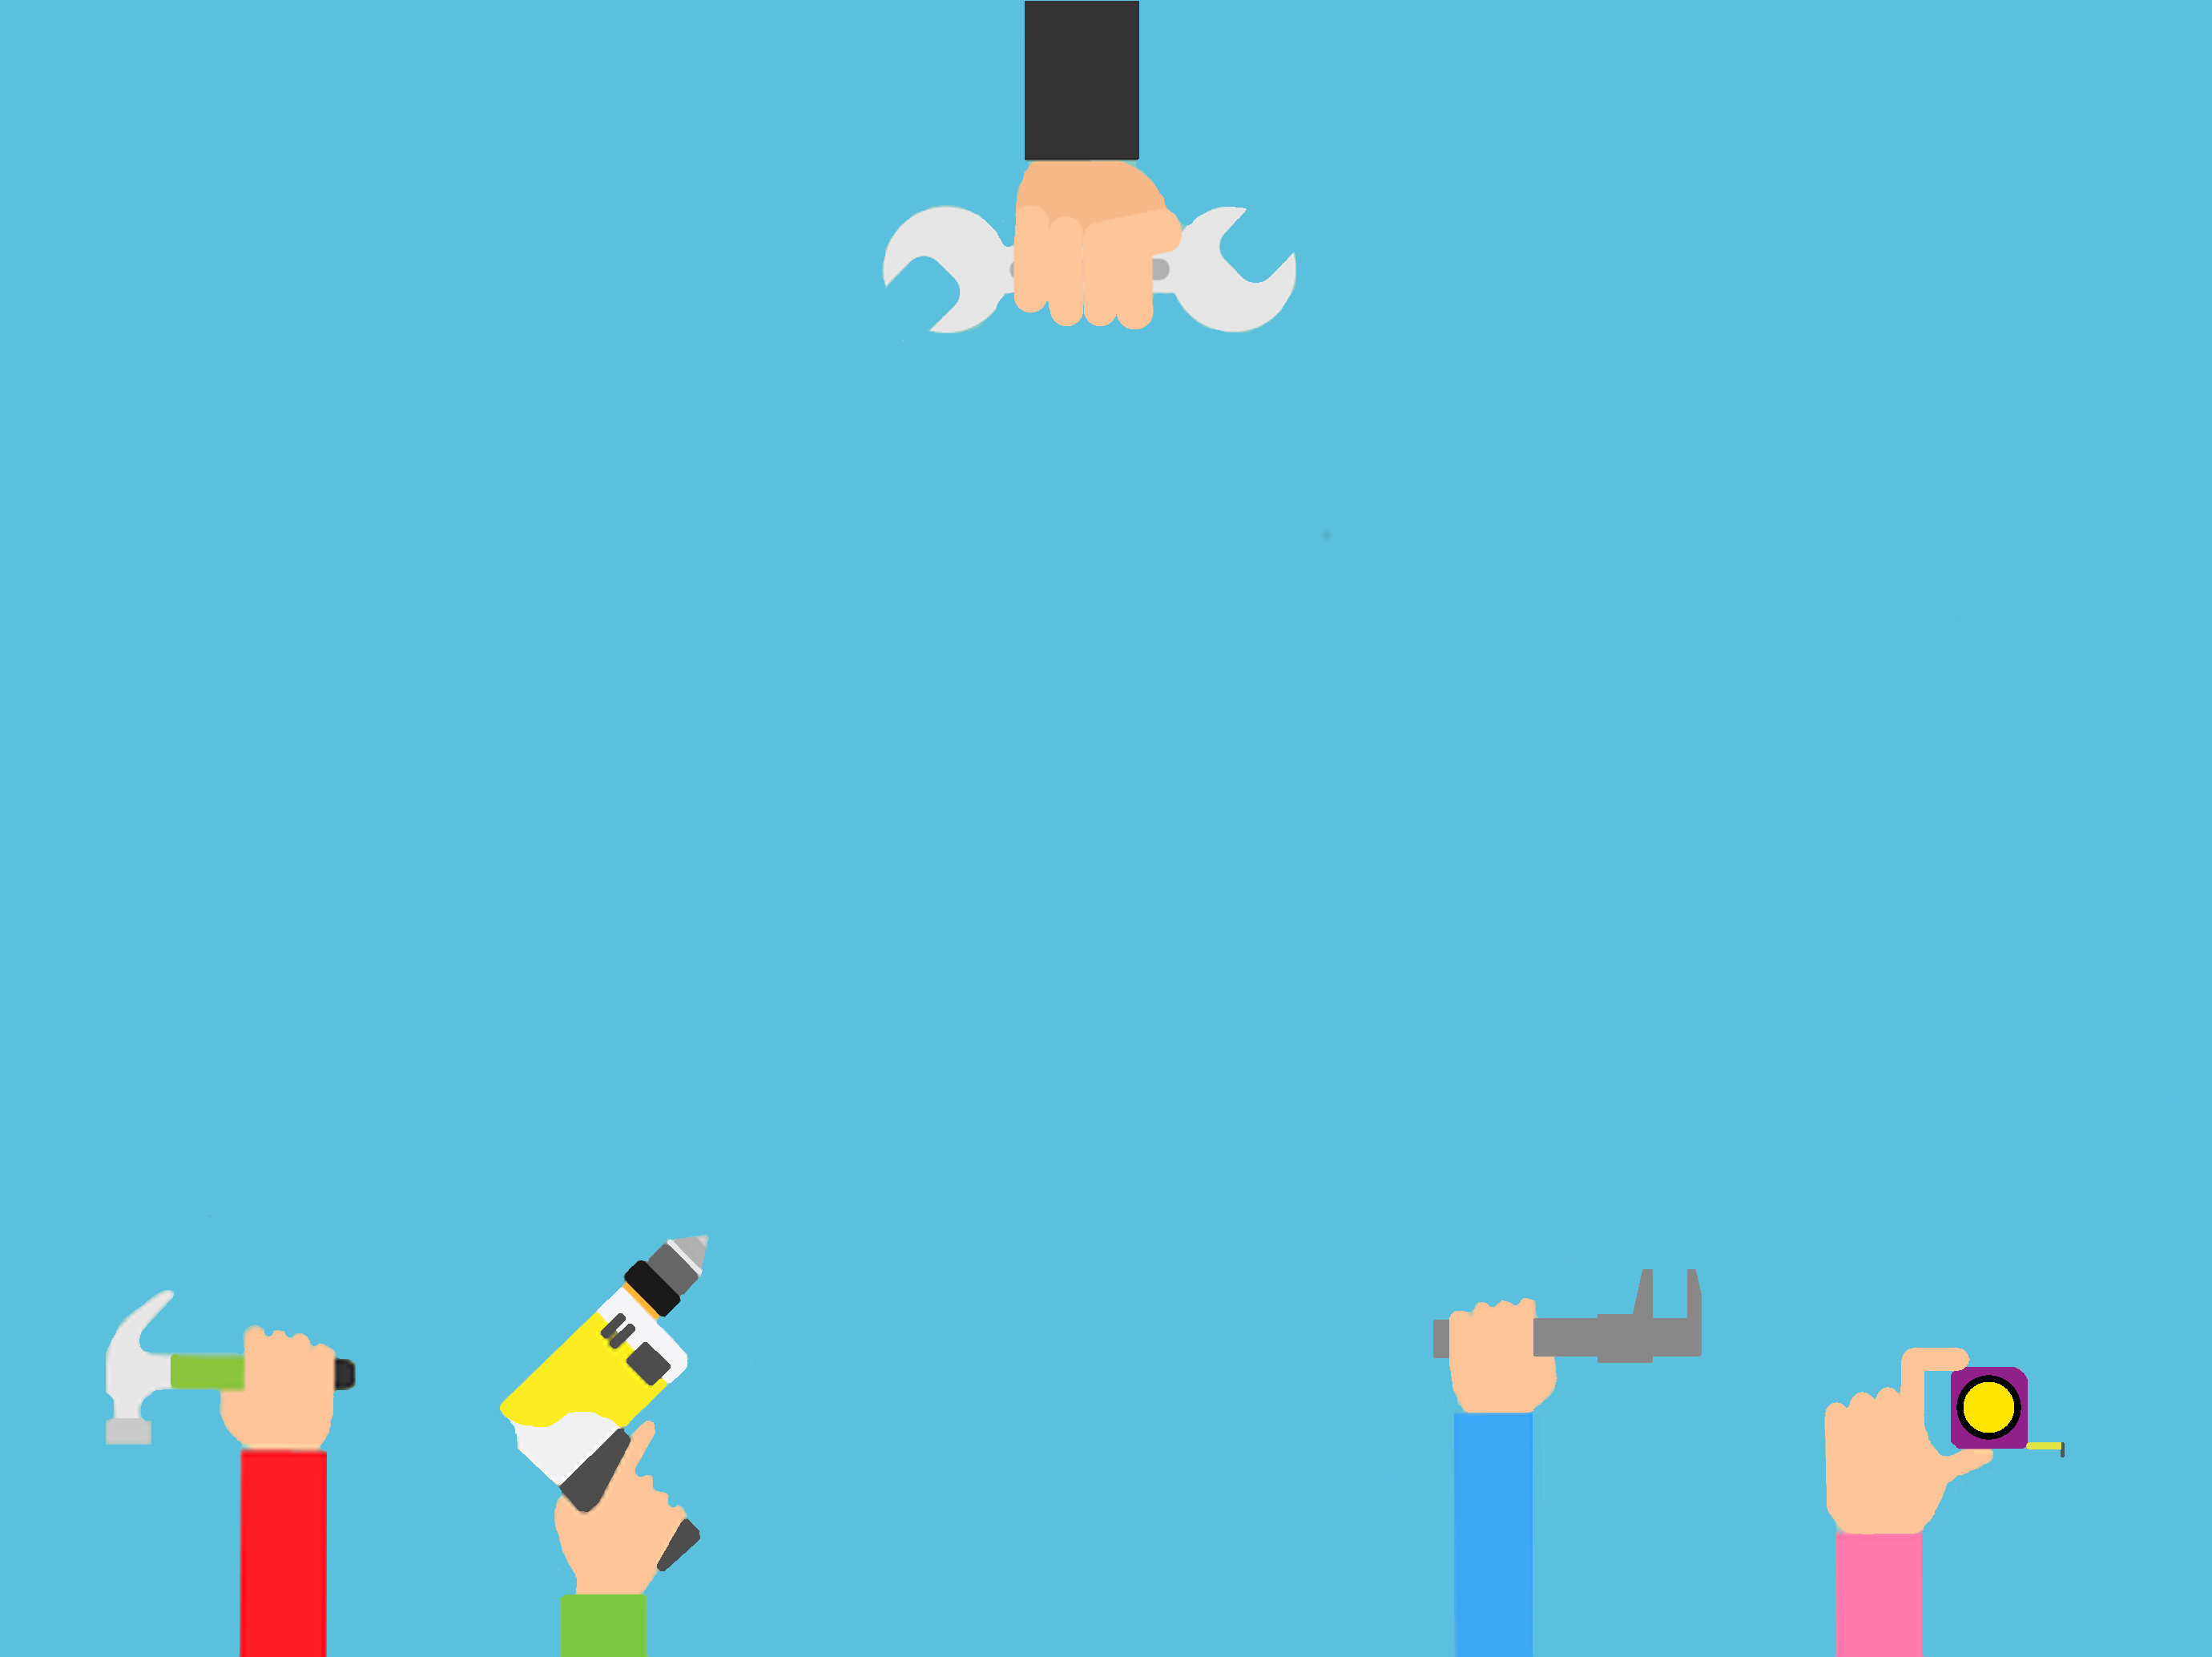
\includegraphics[width=\paperwidth]{../../img/fond}}
\frame{\titlepage}
}



\section{Introduction}

{\frame{
\frametitle{Introduction}

\begin{savoir}
Vous êtes capables :
\begin{itemize}
 \item donner certaines caractéristiques d'un matériau.
\end{itemize}
\end{savoir}

\begin{prob}
Vous devez êtes capables de choisir un procédé de fabrication en fonction:
\begin{itemize}
 \item de la géométrie d'une pièce,
 \item de son matériau,
 \item de la production associée à la pièce.
\end{itemize}
\end{prob}
}}


{\frame{
\frametitle{Plan}
  \tableofcontents[currentsection]
}}

{\frame{
\frametitle{Propriétés et définitions}

\begin{defi}
Le \textbf{moulage} ou \textbf{fonderie} consiste à réaliser des pièces brutes par coulée du métal en fusion dans un moule (représentant l'empreinte de la pièce à obtenir). Le métal en se solidifiant, reproduit les contours et dimensions de l'empreinte du moule. 
\end{defi}

\begin{rem}
\begin{itemize}
 \item \textbf{Utilisation}: Cette technique permet de produire des pièces de formes complexes, la série des pièces est identique et elle permet l'obtention de pièces massives telles que bâtis, volants, etc...
 \item \textbf{Matériaux}: La majorité des matériaux (métalliques et non métalliques) peuvent être moulés.
\end{itemize}
\end{rem}
}}

{\frame{
\frametitle{Types de fonderies}
Dans la spécialisation de la fonderie, on distingue pratiquement les fonderies suivantes :

\begin{itemize}
 \item La nature des métaux et alliages : 
	\begin{itemize}
	\item Fonderie de fonte,
	\item Fonderie d'acier,
	\item Fonderie d'aluminium et ses alliages,
	\item Fonderie de cuivre. Bronzes, laitons, etc.
	\end{itemize}
 \item Selon l'utilisation :
	\begin{itemize}
	\item Fonderie d'art,
	\item Fonderie d'ornement (bijoux),
	\item Fonderie de mécanique industrielle.
	\end{itemize}
 \item Selon le procédé de moulage :
	\begin{itemize}
	\item Moulage en sable (manuel ou mécanique), 
	\item Moulage en carapaces,
	\item Moulage à la cire perdue,
	\item Moulage en coquilles (moule permanent).
	\end{itemize}
\end{itemize}
}}

{\frame{
\frametitle{Types de moule}

\textbf{Le moule non permanent (sable):}
\begin{itemize}
	\item Utilisé une seule fois. Pour extraire la pièce, il faut le détruire. L'empreinte est obtenue par moulage du matériau constitutif autour d'un modèle réalisé en bois ou en métal. 
 \end{itemize}
 
\textbf{Le moule permanent :}
 \begin{itemize}
	 \item Peut servir un grand nombre de fois, il est réalisé en plusieurs parties pour faciliter l'extraction de la pièce. Il est utilisé surtout lorsque la quantité de pièces à couler est importante.
 \end{itemize}
}}

{\frame{
\frametitle{Les procédés en fonction des métaux}
\small
\begin{tabular}{|p{2.5cm}|p{3.5cm}|p{3.5cm}|}
\hline
\begin{itemize}
 \item Fontes : 1100 à 1250°C 
 \item Aciers : 1200 à 1500°C
 \end{itemize} & \begin{itemize}
 \item Moulage en sable avec ou sans noyau,
 \item Moulage en carapace : procédé Croning,
 \item Moulage à la cire perdue 
\end{itemize} & \begin{itemize}
 \item Moulage impossible sans détériorer les coquilles
\end{itemize} \\ \hline 
\begin{itemize}
 \item Laiton : 940°C 
 \item Alpax(Al Si 13) : 610°C
 \item Zamack(Zn Al Cu 4 1) : 610°C
\end{itemize} & \begin{itemize}
 \item Moulage en sable : Grosses pièces, petites séries.
Exemples : \begin{itemize}
 \item Cloches en bronze,
 \item Hélices de bateaux.
\end{itemize}
\end{itemize} & 
\begin{itemize}
 \item Moulage en coquille : 
\begin{itemize}
 \item Pour les grandes séries.
\end{itemize}
 \item Par gravitation ou sous pression.
 Exemples :
\begin{itemize}
 \item Carters (alpax),
 \item Corps de carburateur (zamack). 
\end{itemize}
\end{itemize}\\
\hline 
\end{tabular}
}}

\section{Moulage en sable}

{\frame{
\frametitle{Plan}
  \tableofcontents[currentsection]
}}


{\frame{
\frametitle{Moulage en sable}

\begin{center}
 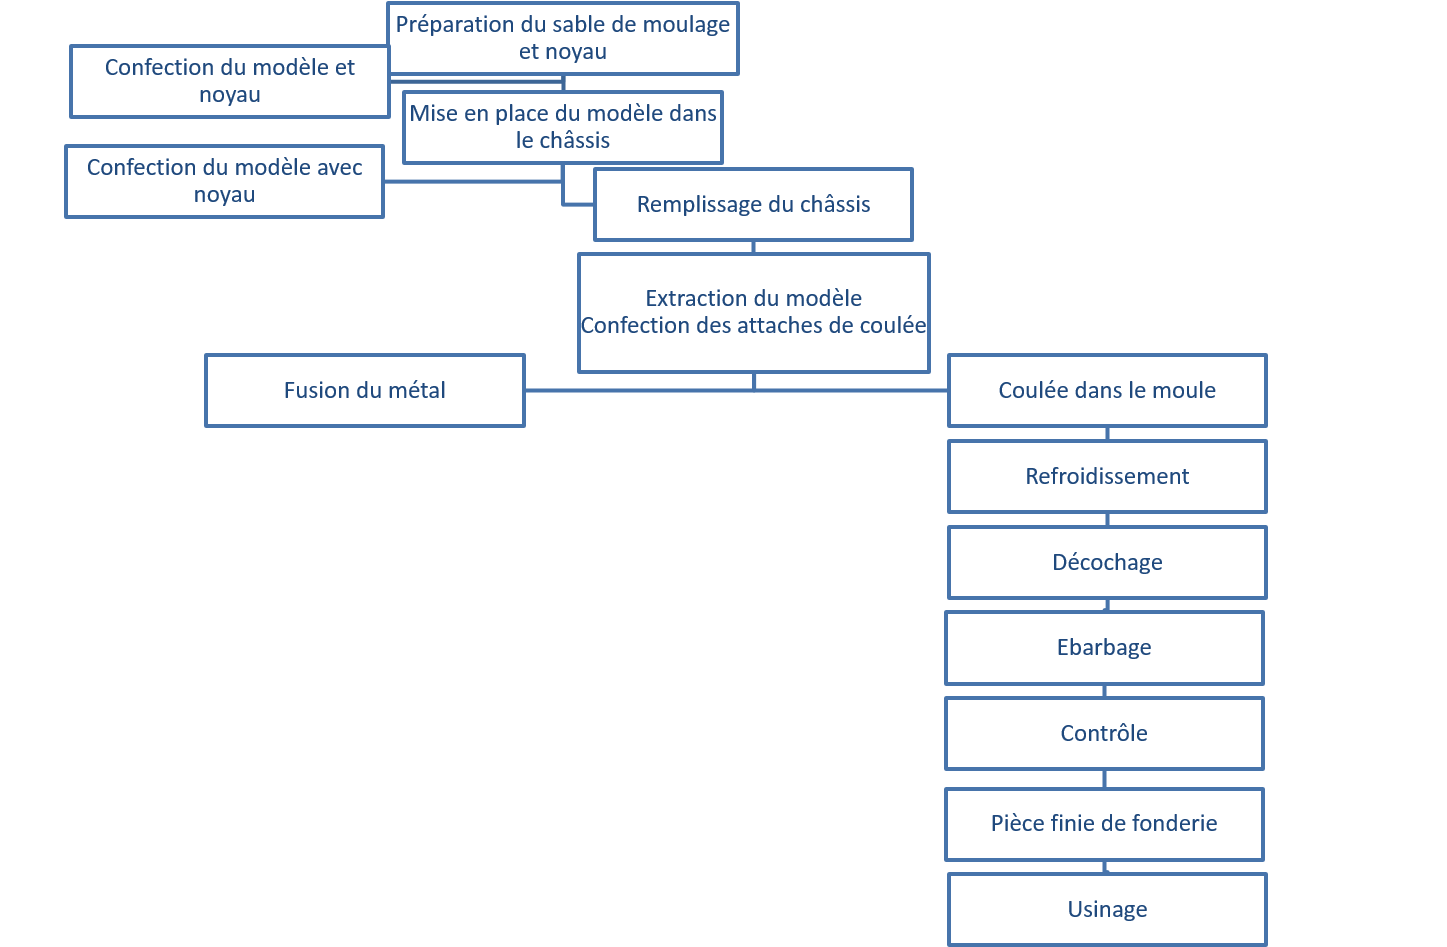
\includegraphics[width=0.9\linewidth]{img/Picture1}
\end{center}
}}

{\frame{
\frametitle{Moulage en sable: Outillage}

\begin{minipage}{0.55\linewidth}
\begin{itemize}
 \item Modèle et noyau,
 \item Châssis,
 \item Sable de moulage,
 \item Métal liquide,
 \item Aiguille (pour la confection de trous d'air),
 \item Truelle (pour rendre lisse la face de joint du moule),
 \item Pillette et fouloir (pour le compactage du sable),
 \item Spatule (pour rendre lisse les différentes surfaces du moule après démoulage,
 \item Mandrin de coulée (pour la confection du trou de coulée),
 \item Marbre (sur lequel s'effectue la préparation du moule).
\end{itemize}
\end{minipage}\hfill
\begin{minipage}{0.4\linewidth}
\begin{center}
 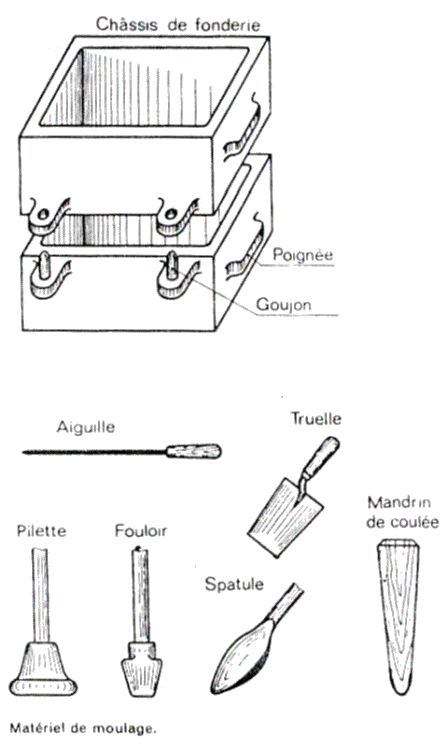
\includegraphics[width=0.9\linewidth]{img/Picture2}
\end{center}
\end{minipage}
}}

{\frame{
\frametitle{Moulage en sable: Le modèle}

Il est construit à partir de la géométrie à réaliser. Il doit tenir compte de:

\begin{minipage}{0.65\linewidth}
\begin{enumerate}
 \item \textbf{L'usinage}: Dans ce cas, la pièce brute doit comporter des surépaisseurs qui seront enlevées durant l'opération d'usinage,
 \item \textbf{Le retrait}: Lors du refroidissement, le métal se contracte, le retrait est la valeur de cette contraction.
 \item \textbf{La dépouille} : Les formes du modèle doivent permettre son extraction du sable sans dégradation du moule. (Angles 3 à 10\%)
\end{enumerate}
\end{minipage}\hfill
\begin{minipage}{0.3\linewidth}
\begin{center}
 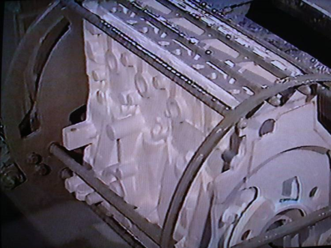
\includegraphics[width=0.9\linewidth]{img/Picture3}
\end{center}
\end{minipage}

\begin{center}
 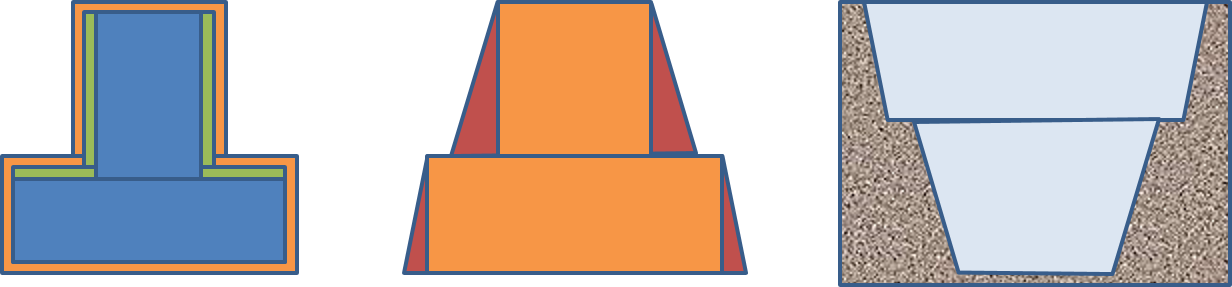
\includegraphics[width=0.8\linewidth]{img/Picture4}
\end{center}
}}

{\frame{
\frametitle{Moulage en sable: Noyau et boîte à noyau}

\begin{minipage}{0.65\linewidth}
Pour obtenir le contour intérieur de la pièce, des noyaux sont placés dans le moule. Ce type de moulage s'impose lorsque les pièces présentent des évidements qu'il serait difficile ou même impossible d'obtenir à partir du moule principal. 
\end{minipage}\hfill
\begin{minipage}{0.3\linewidth}
\begin{center}
 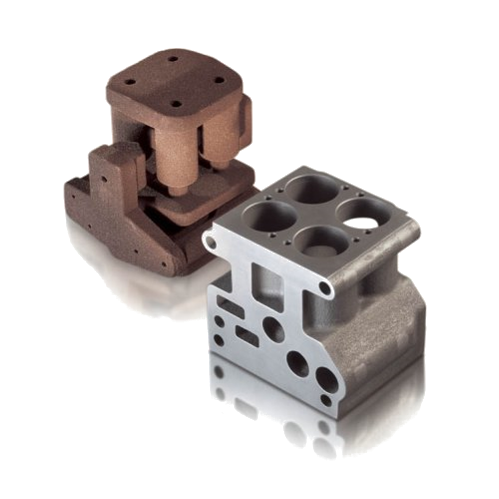
\includegraphics[width=0.9\linewidth]{img/Picture5}
\end{center}
\end{minipage}

\begin{center}
 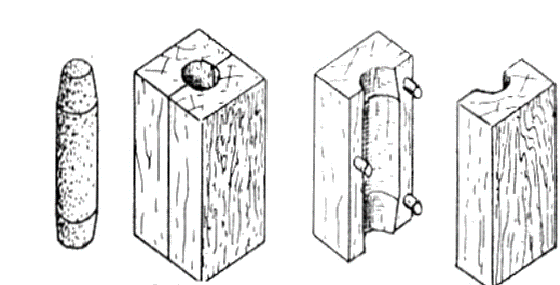
\includegraphics[width=0.7\linewidth]{img/Picture6}
\end{center}
}}

{\frame{
\frametitle{Moulage en sable: Le châssis}

\begin{minipage}{0.55\linewidth}
Cadre rigide (en fonte, en acier ou en aluminium), sans fond, destiné à contenir et à soutenir le sable constituant le moule. Un châssis complet comprend au moins deux parties.
\end{minipage}\hfill
\begin{minipage}{0.4\linewidth}
\begin{center}
 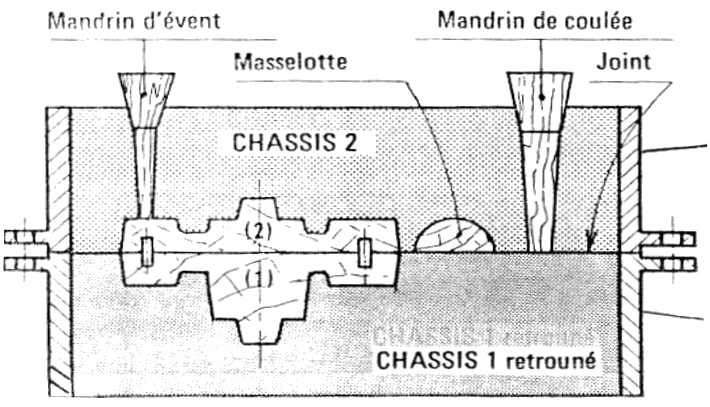
\includegraphics[width=0.9\linewidth]{img/Picture7}
\end{center}
\end{minipage}

\begin{minipage}{0.45\linewidth}
\begin{center}
 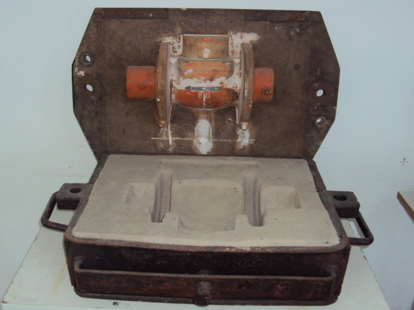
\includegraphics[width=0.8\linewidth]{img/Picture8} \\
Châssis supérieur et modèle supérieur
\end{center}
\end{minipage}\hfill
\begin{minipage}{0.45\linewidth}
\begin{center}
 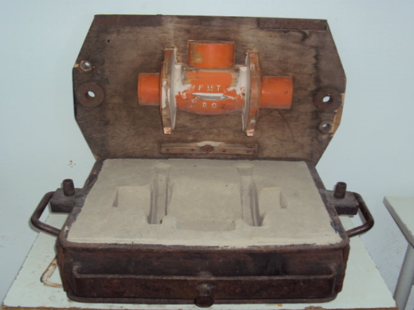
\includegraphics[width=0.8\linewidth]{img/Picture9} \\
Châssis inférieur et modèle inférieur
\end{center}
\end{minipage}
}}

{\frame{
\frametitle{Moulage en sable: Les différents types de moule}

\begin{tabular}{|p{4cm}|p{5cm}|}
\hline
Moule à un élément & 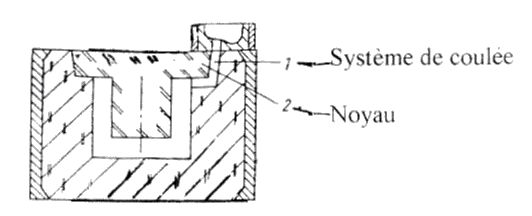
\includegraphics[width=0.9\linewidth]{img/Picture10} \\
\hline
Moule à deux éléments & 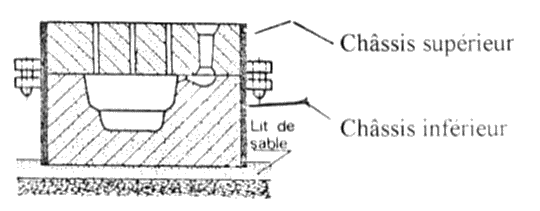
\includegraphics[width=0.9\linewidth]{img/Picture11} \\
\hline
Moule à plusieurs éléments & 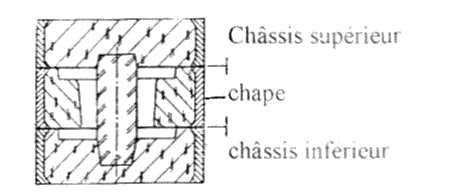
\includegraphics[width=0.9\linewidth]{img/Picture12} \\
\hline
\end{tabular}
}}


{\frame{
\frametitle{Fabrication des moules à la machine}

Il existe différents types de moulage à la machine:
\begin{itemize}
 \item Moulage par pression,
 \item Moulage par secousses,
 \item Moulage par secousses et pression.
\end{itemize}

~\

\begin{minipage}{0.45\linewidth}
\begin{center}
 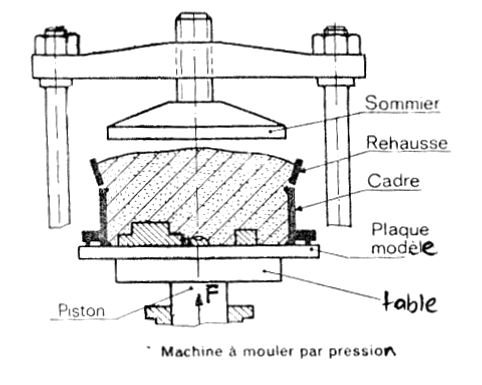
\includegraphics[height=3cm]{img/Picture15}
\end{center}
\end{minipage}\hfill
\begin{minipage}{0.45\linewidth}
\begin{center}
 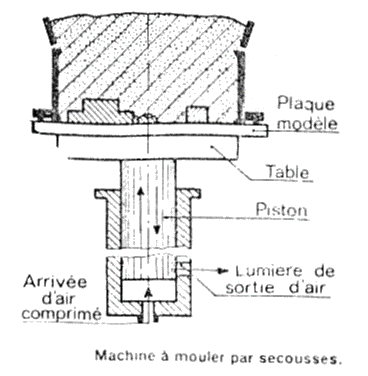
\includegraphics[height=3cm]{img/Picture16}
\end{center}
\end{minipage}
}}

{\frame{
\frametitle{Moulage en sable: Les étapes du moulage}

\begin{minipage}{0.5\linewidth}
\begin{center}
 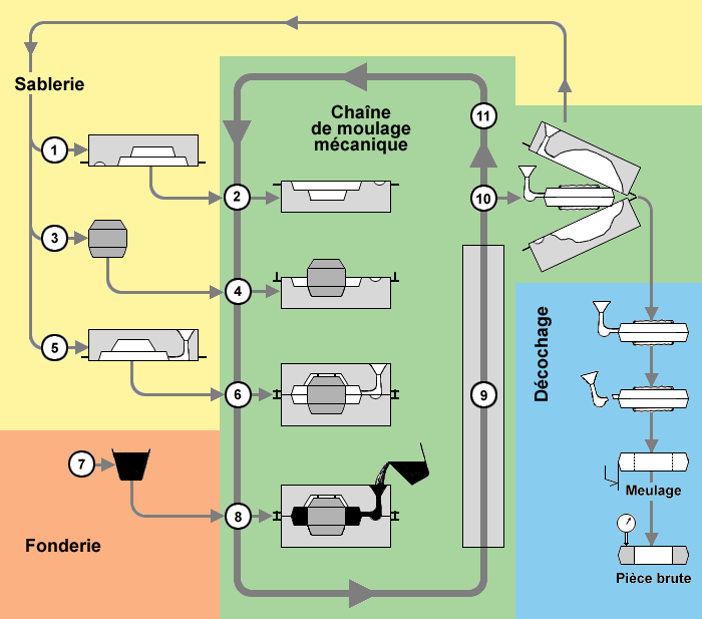
\includegraphics[width=0.9\linewidth]{img/Picture13} \\
 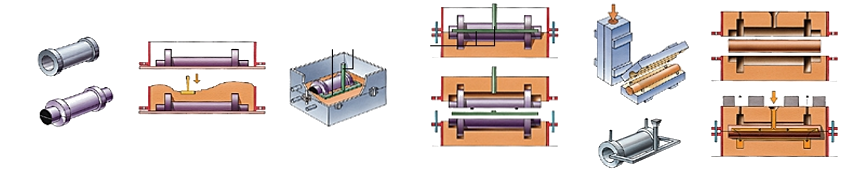
\includegraphics[width=0.8\linewidth]{img/Picture14}
\end{center}
\end{minipage}\hfill
\begin{minipage}{0.45\linewidth}
\ifdef{\public}{\begin{enumerate}[<2->]}{\begin{enumerate}}
 \item \ifdef{\public}{}{\gap}{Fabrication moule inférieur,}
 \item \ifdef{\public}{}{\gap}{Mise en position moule inférieur,}
 \item \ifdef{\public}{}{\gap}{Fabrication des noyaux,}
 \item \ifdef{\public}{}{\gap}{Mise en position des noyaux,}
 \item \ifdef{\public}{}{\gap}{Fabrication moule supérieur,}
 \item \ifdef{\public}{}{\gap}{Mise en position moule supérieur,}
 \item \ifdef{\public}{}{\gap}{Fonte du métal,}
 \item \ifdef{\public}{}{\gap}{Coulée du métal,}
 \item \ifdef{\public}{}{\gap}{Refroidissement,}
 \item \ifdef{\public}{}{\gap}{Démoulage de la pièce,}
 \item \ifdef{\public}{}{\gap}{Recyclage.}
\end{enumerate}
\end{minipage}
}}

\section{Autres procédés}


{\frame{
\frametitle{Plan}
  \tableofcontents[currentsection]
}}

{\frame{
\frametitle{Moulage avec moule métallique}

\begin{minipage}{0.65\linewidth}
\textbf{Moulage en coquille} \\
\begin{itemize}
 \item Le moulage en coquille est un procédé qui permet de couler par gravité le métal en fusion directement dans un moule métallique en fonte ou en acier appelé coquille. 
 \item Ce type de moulage est destiné pour la réalisation de pièces complexes en métaux et alliages ferreux (fonte grise et acier) et alliages non ferreux à point de fusion relativement bas, bronzes (10 à 13\% Zinc), Al-Si possédant de bonnes propriétés de fonderie, AI-Si-Cu, Al-Cu (4 à 12\% Cu). 
\end{itemize}
\end{minipage}\hfill
\begin{minipage}{0.3\linewidth}
\begin{center}
 
\includegraphics[height=3cm]{img/Picture17}
\end{center}
\end{minipage}

\textbf{Moulage sous pression} \\
Dans ce procédé, le métal liquide est injecté dans le moule de la machine à mouler sous pression (30 à 100 MPA). Ce procédé permet d'obtenir des pièces ayant une configuration très complexe avec des dimensions très précises, ce qui permet de supprimer partiellement ou totalement les opérations d'usinage.
}}

{\frame{
\frametitle{Moulage en carapace: Procédé Croning}

\begin{minipage}{0.75\linewidth}
Le moulage en carapace ressemble au moulage mécanique en sable, dans ce cas, le métal liquide est coulé dans un moule constitué de deux coquilles appelées carapaces ou masques.
\end{minipage}\hfill
\begin{minipage}{0.2\linewidth}
\begin{center}
 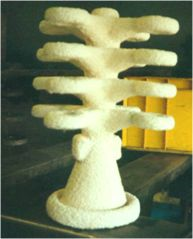
\includegraphics[height=3cm]{img/Picture18}
\end{center}
\end{minipage}

\begin{minipage}{0.25\linewidth}
\begin{center}
 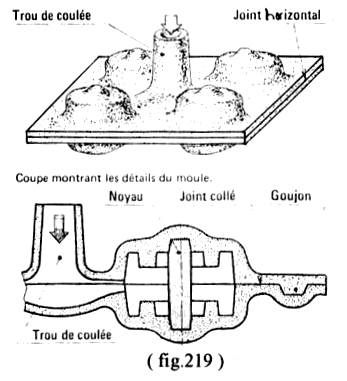
\includegraphics[width=0.9\linewidth]{img/Picture19}
\end{center}
\end{minipage}\hfill
\begin{minipage}{0.7\linewidth}
Fabrication d'une carapace : 
\begin{enumerate}
 \item Préparer du sable de moulage (séchage, additions),
 \item Chauffer de la plaque modèle (réversible),
 \item Verser sur la plaque-modèle chauffée, un mélange de grains de silice (sable) et de résine thermodurcissable,
 \item Retourner l'ensemble caisson et plaque modèle, 
 \item Placer la plaque modèle et la carapace dans un four.
\end{enumerate}
\end{minipage}
}}

{\frame{
\frametitle{Moulage à la cire perdue}

\begin{minipage}{0.25\linewidth}
\begin{center}
 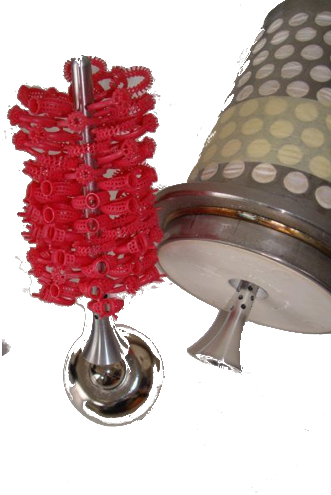
\includegraphics[width=0.9\linewidth]{img/Picture20}
\end{center}
\end{minipage}\hfill
\begin{minipage}{0.7\linewidth}
Fabrication d'une carapace : 

Ce procédé permet de s'affranchir du démoulage du modèle et des contraintes qui vont avec. \\
Principe du moulage à la cire perdue:
\begin{itemize}
 \item Le moule est construit autour d'un modèle en cire, lequel ensuite est éliminé par fusion pour libérer l'empreinte formée,
 \item Il faut donc dans ce cas un modèle par moule,
 \item Les modèles en cire sont moulés ou bien fabriqués par prototypage rapide.
\end{itemize}
\end{minipage}
}}

{\frame{
\frametitle{Les défauts du moulage}

\begin{itemize}
 \item Défauts affectant la surface
 \begin{enumerate}
  \item Défauts: Bavures, épaississements, saillies (dans le plan de joint)
  \item Causes: décollement (détachement) dans le moule, fissuration du sable, arrachements de sable, écrasement du moule.
  \item Les criques, fêlures et ruptures sont dues aux tensions internes provenant des retraits de refroidissement 
  \item D'autres types de défauts pouvant exister sur les pièces moulées sont : 
   \begin{itemize}
   \item Rugosité superficielle. 
   \item Différence de forme et de dimension. 
   \item Pièce moulée incomplète,
   \item Brûlures du sable (haute température)
   \end{itemize}
  \end{enumerate}
 \item Défauts affectant la masse ou le volume
 \begin{enumerate}[a.]
  \item Les inclusions d'air,
  \item Les soufflures,
  \item Les retassures.
 \end{enumerate}
\end{itemize}
}}

{\frame{
\frametitle{Les défauts du moulage}

\begin{center}
 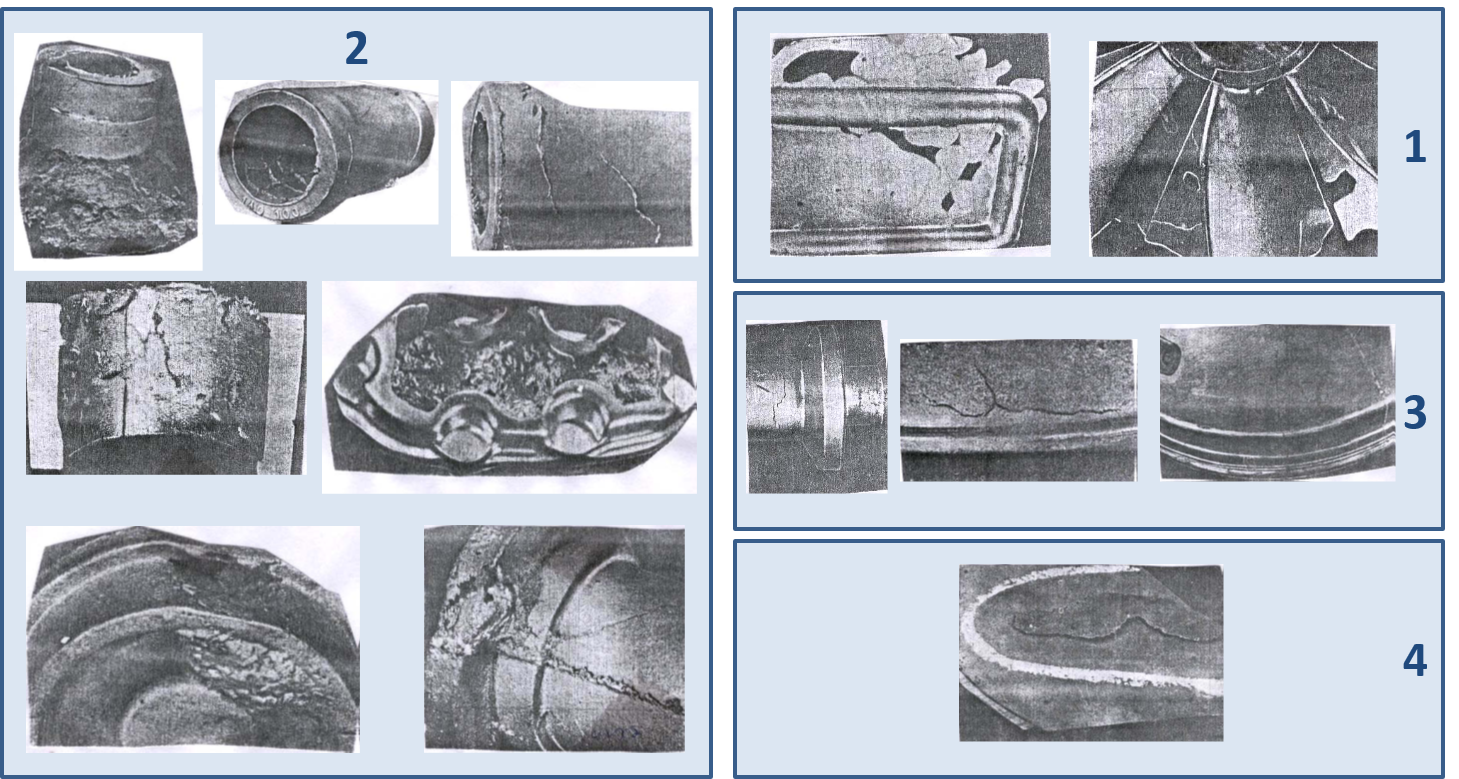
\includegraphics[width=0.9\linewidth]{img/Picture21}
\end{center}

}}

{\frame{
\frametitle{Les défauts du moulage}

\begin{center}
 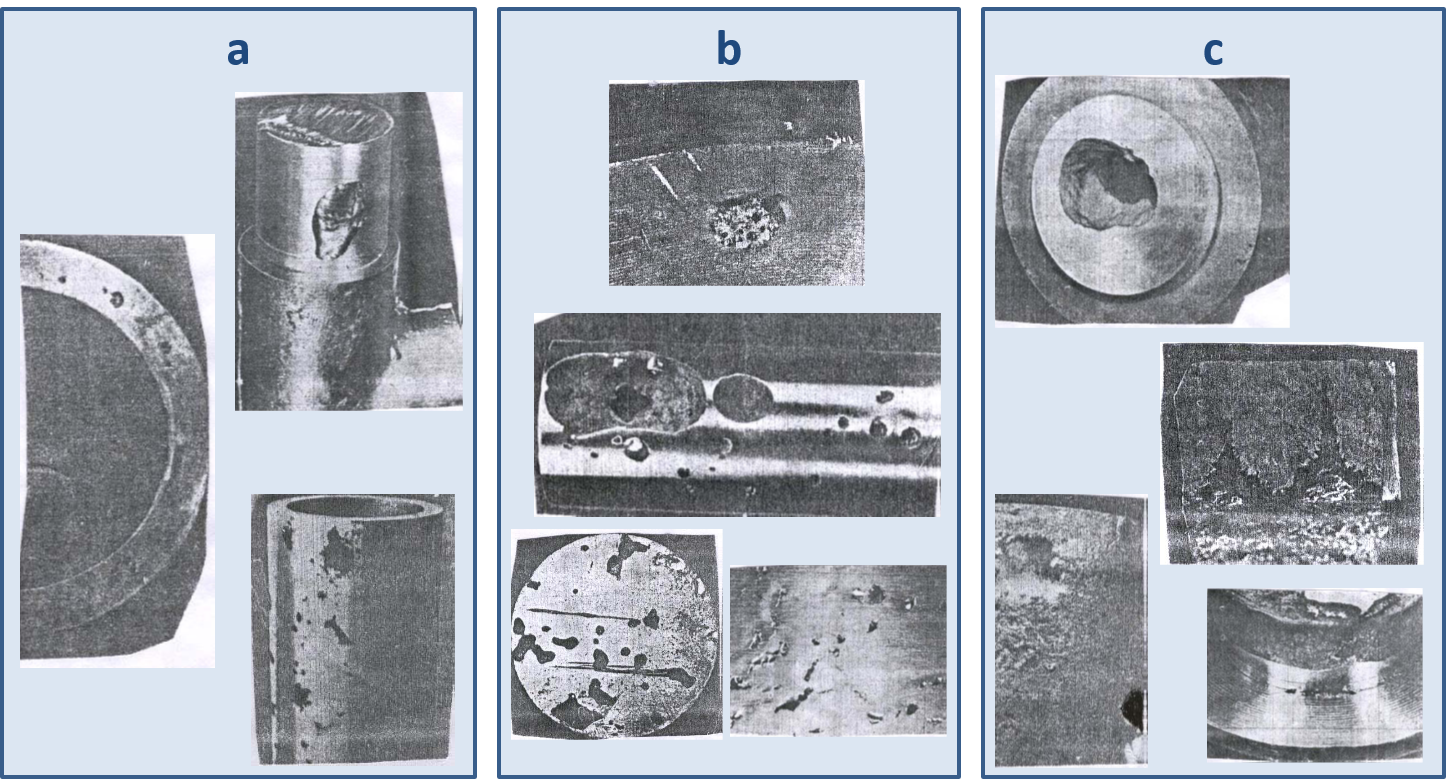
\includegraphics[width=0.9\linewidth]{img/Picture22}
\end{center}
}}

\section{Injection plastique}

{\frame{
\frametitle{L'injection plastique: Principe}

\begin{minipage}{0.35\linewidth}

\includegraphics[width=0.9\linewidth]{img/Picture23}
\end{minipage}\hfill
\begin{minipage}{0.6\linewidth}
L'injection des polymères permet d'obtenir en une seule opération des pièces finies, de formes complexes, dans une gamme de poids de quelques grammes à plusieurs kilogrammes.
\end{minipage}

~\

\begin{minipage}{0.6\linewidth}
\begin{enumerate}
 \item Vis de plastification contrôlée par la presse,
 \item Trémie d'alimentation,
 \item Buse d'injection,
 \item Partie fixe du moule,
 \item Empreinte/pièce,
 \item Partie Mobile du moule.
\end{enumerate}
\end{minipage}\hfill
\begin{minipage}{0.35\linewidth}
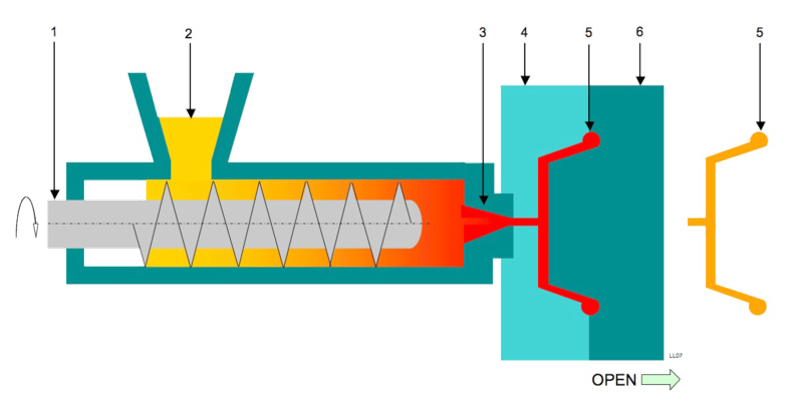
\includegraphics[width=0.9\linewidth]{img/Picture24}
\end{minipage}
}}

{\frame{
\frametitle{L'injection plastique: Outillage}

\begin{minipage}{0.35\linewidth}
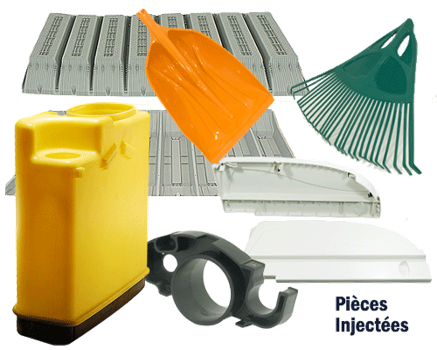
\includegraphics[width=0.9\linewidth]{img/Picture25}
\end{minipage}\hfill
\begin{minipage}{0.6\linewidth}
Un moule, doit remplir plusieurs fonctions :
\begin{itemize}
 \item fonction mise en forme,
 \item fonction alimentation,
 \item fonction régulation,
 \item fonction refroidissement de la pièce,
 \item fonction éjection.
\end{itemize}
\end{minipage}

\begin{minipage}{0.35\linewidth}
\begin{enumerate}
 \item Le moule,
 \item Les éjecteurs,
 \item Les plaques dévêtisseuses.
\end{enumerate}
\end{minipage}\hfill
\begin{minipage}{0.35\linewidth}
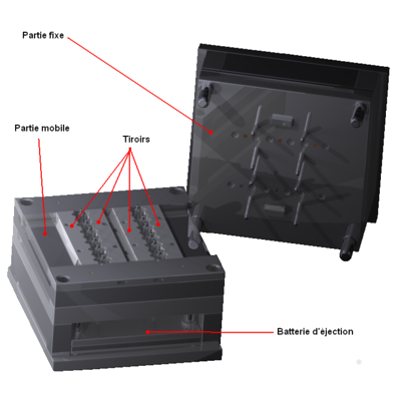
\includegraphics[width=0.9\linewidth]{img/Picture26}
\end{minipage}
}}	

{\frame{
\frametitle{Problématiques liées à l'injection plastique}

\begin{minipage}{0.48\linewidth}
\textbf{Défauts des pièces injectées}
\begin{itemize}
 \item Retassures,
 \item Jet libre,
 \item Défauts en ligne de soudure,
 \item Cernes et sillons,
 \item Entrainement d'air,
 \item Sous-dosage et surdosage,
 \item Bulles et effets fontaine,
 \item Commutation précoce et commutation tardive,
 \item Conséquence d'une commutation décalée,
\end{itemize}
\end{minipage}\hfill
\begin{minipage}{0.48\linewidth}
\begin{itemize}
 \item Défauts dimensionnels,
 \item Matière humide avant transformation,
 \item Incorporation d'éléments étranger et mauvais mélange,
 \item Combustion ou effet diesel - carbonisation.
\end{itemize}
~\
\textbf{Problèmes de démoulage}
\begin{itemize}
 \item Marquage des éjecteurs,
 \item La pièce reste coincée dans le moule ? dégradation mécanique de la pièce,
 \item Tirage de fil.
\end{itemize}
\end{minipage}
}}

\section{Règles de tracé}

{\frame{
\frametitle{Variations d'épaisseur}

\begin{itemize}
 \item Ne pas dépasser un accroissement de 60 \% sur 10 mm.
\end{itemize}

\begin{center}
 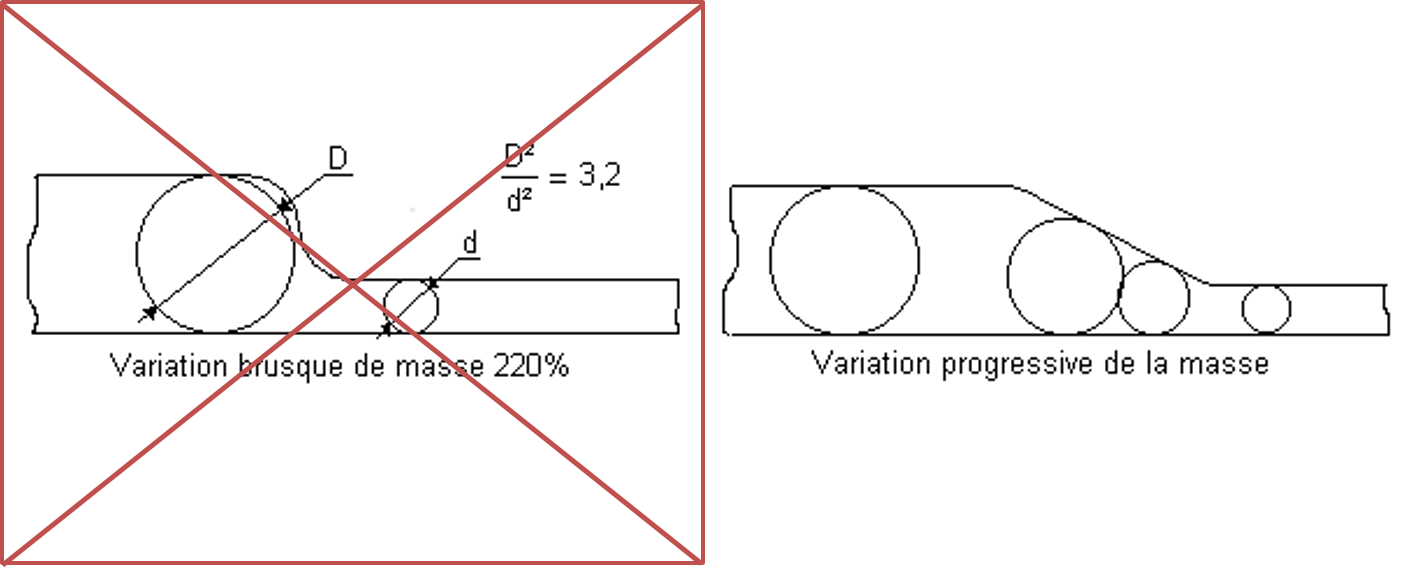
\includegraphics[width=0.9\linewidth]{img/Picture27}
\end{center}
}}

{\frame{
\frametitle{Raccordement d'épaisseurs différentes}

\begin{itemize}
 \item Lorsque l'écart des épaisseurs $E-e$ ne dépasse pas $\dfrac{E}{3}$ le raccordement peut se faire suivant un rayon égal à $E$ sur l'une des faces ou sur les deux faces avec un rayon égal à $\dfrac{E}{2}$,
 \item Si l'écart est plus élevé, le raccordement doit être fait avec une pente à 20\%.
\end{itemize}

\begin{center}
 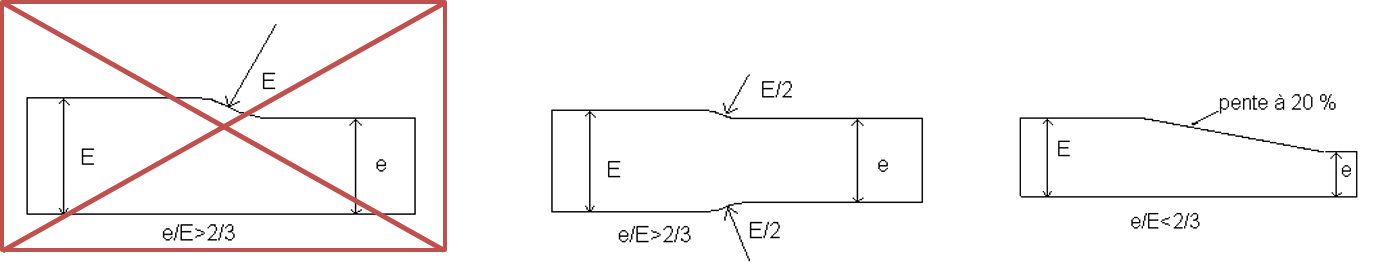
\includegraphics[width=0.9\linewidth]{img/Picture28}
\end{center}
}}

{\frame{
\frametitle{Raccordement de parois}

\begin{itemize}
 \item Un raccordement en L à angle vif pose à la fois la question de la surépaisseur diagonale et celle du point chaud créé dans le moule sur l'arête intérieure. La diffusion de la chaleur du métal vers le moule est élevée vers l'extérieur et plus limitée au contraire vers l'intérieur où se produisent criques et retassures
\end{itemize}

\begin{itemize}
 \item Un arrondi mal adapté déplace la retassure vers l'extérieur,
 \item $R=E+e$,
 \item $r=\dfrac{E+e}{2}$
\end{itemize}

\begin{center}
 
\includegraphics[width=0.9\linewidth]{img/Picture29}
\end{center}
}}

{\frame{
\frametitle{Allègement des parties massives}

\begin{itemize}
 \item L'allègement des parties massives est également à prendre en compte dans le tracé de la pièce pour contribuer à l'homogénéité des épaisseurs.
\end{itemize}

\begin{center}
 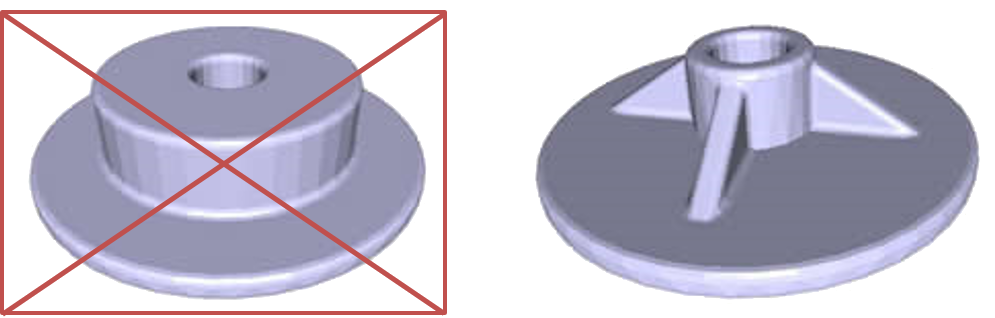
\includegraphics[width=0.9\linewidth]{img/Picture30}
\end{center}
}}

{\frame{
\frametitle{Éviter les tensions}

\begin{minipage}{0.65\linewidth}
\begin{itemize}
 \item Le retrait peut engendrer des tensions dans la pièce de fonderie, soit du fait des différences d'épaisseurs entraînant des différences de température et de contraction, soit à cause des formes de la pièce ou du moule.
\end{itemize}
\end{minipage}\hfill
\begin{minipage}{0.3\linewidth}
\begin{center}
 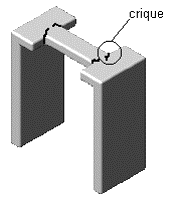
\includegraphics[width=0.9\linewidth]{img/Picture31}
\end{center}
\end{minipage}

\begin{center}
 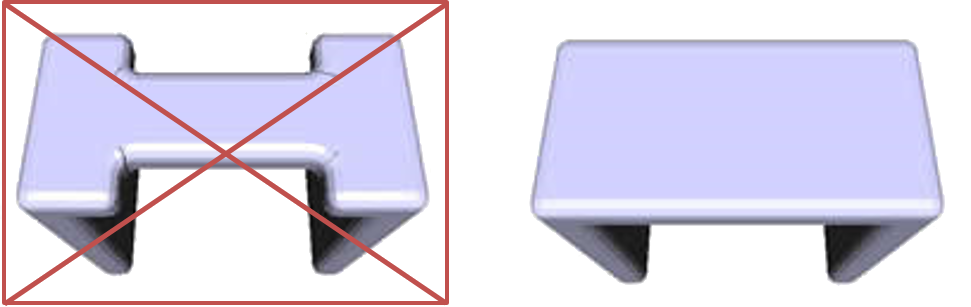
\includegraphics[width=0.9\linewidth]{img/Picture32}
\end{center}
}}

{\frame{
\frametitle{Dépouilles}

\begin{itemize}
 \item Pour les \textbf{moules en sable}, la dépouille permet le démoulage du modèle sans détérioration de l'empreinte.
 \item Pour les \textbf{moules permanents} (moulage en coquille par gravité, moulage basse pression ou moulage par pression), la dépouille est nécessaire pour extraire la pièce moulée de l'empreinte.
\end{itemize}

\begin{center}
 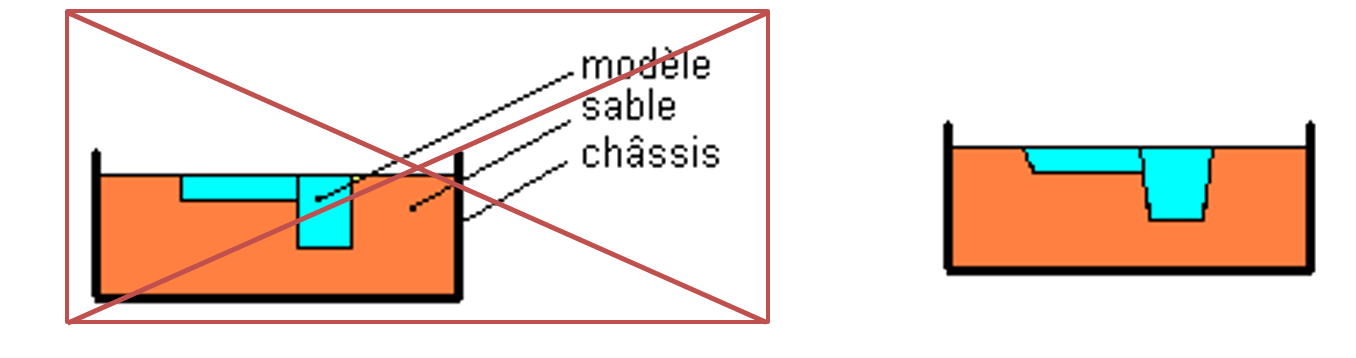
\includegraphics[width=0.9\linewidth]{img/Picture33}
\end{center}
}}

{\frame{
\frametitle{Plan de joint}

\begin{itemize}
 \item En général, le démoulage s'effectue \textbf{perpendiculairement} au plan de joint. La géométrie de la pièce doit permettre ce démoulage,
 \item Il est avantageux de reporter l'empreinte dans \textbf{une seule partie} du moule. La dépouille d'un seul côté est plus importante, mais le modèle en une seule partie est plus économique.
\end{itemize}

\begin{center}
 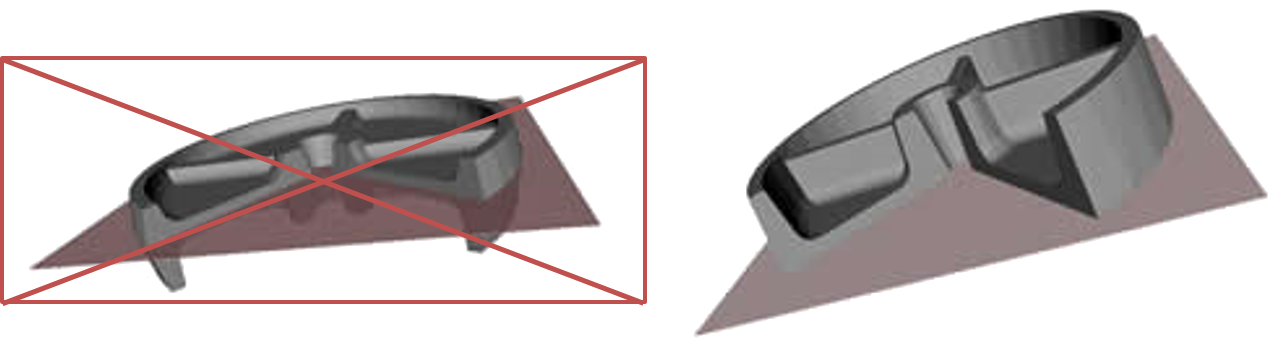
\includegraphics[width=0.9\linewidth]{img/Picture34}
\end{center}
}}

{\frame{
\frametitle{Noyau}

\begin{itemize}
 \item Le noyau doit être convenablement mis en place dans le moule. Ses assises, ou portées, demandent beaucoup de précision.
\end{itemize}

\begin{center}
 
\includegraphics[width=0.9\linewidth]{img/Picture35}
\end{center}
}}

{\frame{
\frametitle{Résistance à la compression}

\begin{itemize}
 \item Imposer que la contrainte maximale soit celle de compression.
\end{itemize}

\begin{center}
 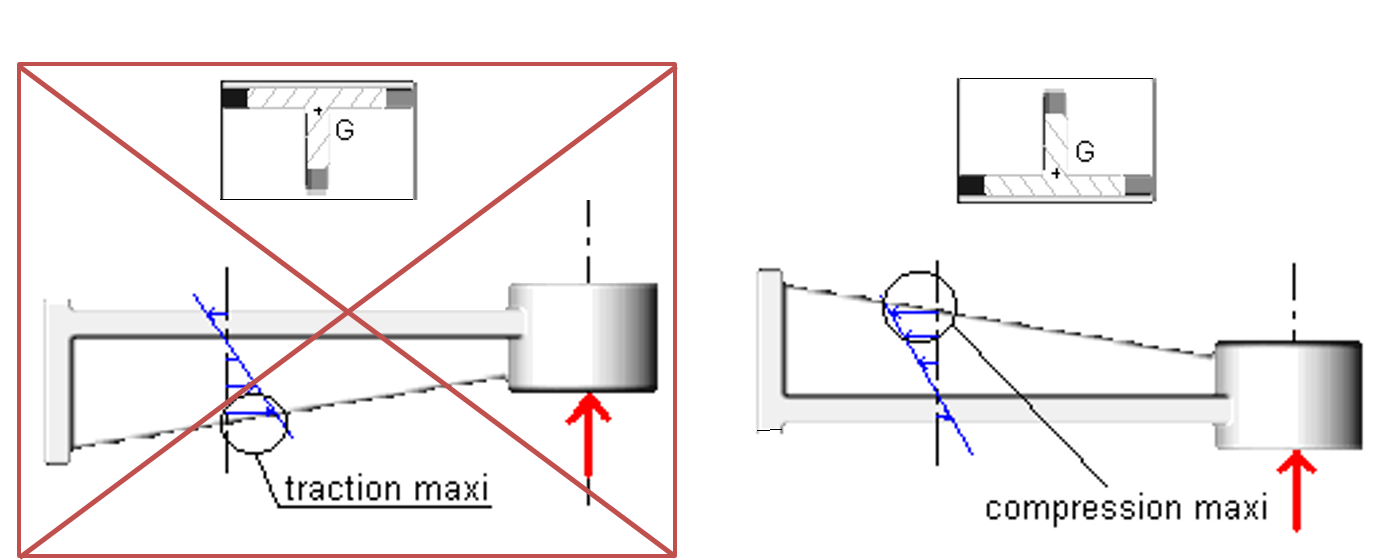
\includegraphics[width=0.9\linewidth]{img/Picture36}
\end{center}
}}

{\frame{
\frametitle{Surépaisseur d'usinage}

\begin{itemize}
 \item Le tracé de la pièce de fonderie doit tenir compte des surépaisseurs d'usinage. Elles apparaissent sur les surfaces fonctionnelles.
\end{itemize}

\begin{center}
 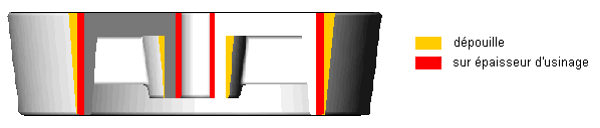
\includegraphics[width=0.9\linewidth]{img/Picture37}
\end{center}
}}

{\frame{
\frametitle{Etat de surface}

\begin{itemize}
 \item L'état de surface est fonction du procédé de moulage et de l'alliage : 
	\begin{itemize}
 	\item matériau de moulage (composition, granulométrie),
dispositifs modifiant localement l'empreinte du moule (enduits, couches, sables de contact),
	\item comportement de l'alliage à l'interface moule-alliage,
	\item conception du moule (bavures, défauts de surface).
	\end{itemize}
 \item La \textbf{rugosité} d'une surface brute n'est spécifiée que sur des surfaces fonctionnelles, elle peut conditionner le choix d'un procédé de moulage.
\end{itemize}

\begin{center}
 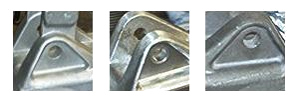
\includegraphics[width=0.9\linewidth]{img/Picture38}
\end{center}
}}

{\frame{
\frametitle{Conclusion}

\begin{savoir}
Vous êtes capables :
\begin{itemize}
 \item de concevoir une pièce moulée,
 \item de représenter les éléments de moulage.
\end{itemize}
\end{savoir}

\begin{prob}
Vous devez êtes capables :
 \begin{itemize}
 \item de concevoir une pièce moulée.
 \end{itemize}
\end{prob}
}}


\end{document}